\section{M0 in detail}
\label{app:supporting}

\subsection{The exact sampler on M0}
\label{app:posteriors}

\paragraph{Coverage.} We read coverage off the ranks of \cref{fig:calibration}A, for central credible intervals at five
levels from 50\% to 99\%. In \pn{vseven.cov} parameter--level pairs the coverage is
inside the binomial 95\% band. One or two misses over 30 pairs are expected by chance.
The one miss is the decay rate at 99\%, where $L = \pn{mzero.L}$ draws per chain give
the coarsest ranks.

\paragraph{A production-length chain matches the reference.} One chain of the
length we used in the calibration runs is not distinguishable from the reference on
any marginal (\cref{fig:calibration}B). The means differ by at most
\pn{ften.dmean} reference standard deviations, and the ratio of standard deviations
is between \pn{ften.sdlo} and \pn{ften.sdhi}. This chain cost \pn{ften.cpuh}
CPU-hours. Its effective sample size is low, so this comparison has low resolving power.
The production chain separates the FBA constant from its matched null by a small
margin, \pn{ften.fbamargin} standard deviations.

\begin{figure*}[t]
\centering
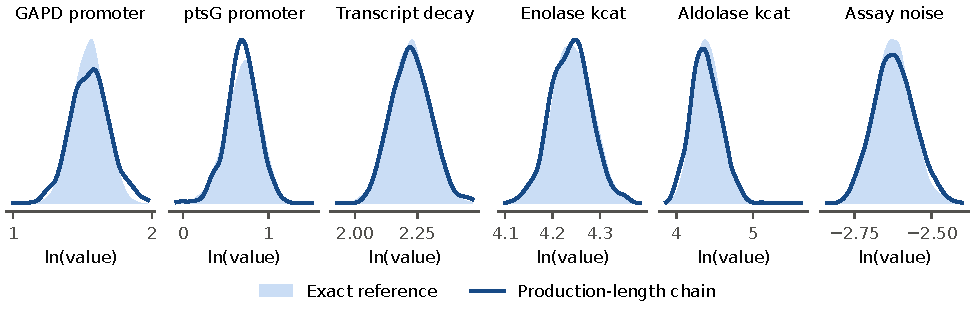
\includegraphics[width=\linewidth]{fig_calibration.pdf}
\caption{\textbf{The exact sampler on M0.} A: rank-ECDF of the truth over \pn{vseven.R}
prior-drawn datasets, against simultaneous bands at a joint level of 95\%. The grey region is the band, and the line is the rank-ECDF minus the fractional rank. B: marginal posteriors of the natural log of each parameter on one dataset: the reference as a filled blue density, and a production-length chain as the orange line.}
\label{fig:calibration}
\end{figure*}

\subsection{The mixed route: holding $S$ fixed}
\label{app:sfixed}

$S$ is computed once, at a reference parameter value.
A sensitivity check re-estimated it at the posterior mean on three datasets. The
marginals moved detectably on \pn{mix.ksfired} comparisons, each by at most
\pn{mix.ksmargin} standard deviations over its floor. Against a matched null of two
identical fits, two of the five are about twice the noise, one is 1.3 times it, and
two are within it.

\subsection{The mean-field swap: goodness check and limit}
\label{app:swap}

\paragraph{The goodness check.} The check as first written fails a description known to be correct
in about half of all cases: a correct description passes only
\pn{jg.kgnulllo}--\pn{jg.kgnullhi}\% of the time. We therefore compare the check
with its own null distribution. With $\delta$, the mean field falls inside the
null's 95\% range at \pn{jg.deltain} targets, against \pn{jg.mfin} without
$\delta$.

\paragraph{The mean-field model is the limit of the hybrid's pinned path.} The hybrid exchanges state every second. When the driver follows the mean-field path, this path converges to the one-ODE mean-field model as the step shrinks. That is a limit of the deterministic path, and not of the stochastic hybrid, whose gap is the subject of \cref{sec:jensen}. Extrapolated to a zero step, the two agree to
\pn{rii.maxdelta} in log concentration at all five test parameter sets. One
mean-field solve takes \pn{rii.mzero}\,s on M0 and \pn{rii.corealo}--\pn{rii.coreahi}\,s
on the full reduced model.

\subsection{M0's crossed comparison}
\label{app:crossed}

\Cref{tab:crossed} gives the coverages and widths that \cref{fig:crossed} plots.

\begin{table*}[t]
\caption{\textbf{M0's crossed comparison.} \textbf{Scored} against the truth over \pn{vseven.R}
datasets, as percentage coverage $\pm$ one standard error. Width is the median ratio of
the 90\% interval to that of the exact posterior with the hybrid. The references at these
sizes are \pn{pred.ref50}\% and \pn{pred.ref90}\%. The $\Delta Q$ columns do not meet the
sizing rules in \cref{sec:predm0}, so they are not clean calibration numbers.}
\label{tab:crossed}
\centering
\small
\begin{tabular}{@{}llcccccc@{}}
\toprule
& & \multicolumn{3}{c}{$Q$, lactate export} & \multicolumn{3}{c}{$\Delta Q$, knockdown effect} \\
Posterior & Forward & 50\% & 90\% & Width & 50\% & 90\% & Width \\
\midrule
Exact & Hybrid & \pn{pred.q.eh.c} & \pn{pred.q.eh.n} & 1 & \pn{pred.d.eh.c} & \pn{pred.d.eh.n} & 1 \\
Exact & Mean field & \pn{pred.q.em.c} & \pn{pred.q.em.n} & \pn{pred.q.em.w} & \pn{pred.d.em.c} & \pn{pred.d.em.n} & \pn{pred.d.em.w} \\
Exact & Mean field $+\,\delta$ & \pn{pred.q.ed.c} & \pn{pred.q.ed.n} & \pn{pred.q.ed.w} & \pn{pred.d.ed.c} & \pn{pred.d.ed.n} & \pn{pred.d.ed.w} \\
Mixed & Hybrid & \pn{pred.q.mh.c} & \pn{pred.q.mh.n} & \pn{pred.q.mh.w} & \pn{pred.d.mh.c} & \pn{pred.d.mh.n} & \pn{pred.d.mh.w} \\
Mixed & Mean field & \pn{pred.q.mm.c} & \pn{pred.q.mm.n} & \pn{pred.q.mm.w} & \pn{pred.d.mm.c} & \pn{pred.d.mm.n} & \pn{pred.d.mm.w} \\
Mixed & Mean field $+\,\delta$ & \pn{pred.q.md.c} & \pn{pred.q.md.n} & \pn{pred.q.md.w} & \pn{pred.d.md.c} & \pn{pred.d.md.n} & \pn{pred.d.md.w} \\
\bottomrule
\end{tabular}
\end{table*}

\subsection{What the mean-field swap costs}
\label{sec:jensen}

The mixed route rests on the mean-field swap, which replaces the stochastic gene expression with its mean. The
means of transcripts and proteins are exact, but metabolism is nonlinear. A
metabolism fed the mean drain differs from the mean over cells of metabolisms fed
their own drains. The difference is a Jensen gap.

The gap is largest for GTP, where the mean field sits
\pn{jg.gtplo}--\pn{jg.gtphi}\% below the population mean. We traced it to
cell-to-cell variation in the drains. When every cell receives the mean field's
drains, the gap closes. At our three test parameter sets, the enzyme counts, the per-cell feedback and the clip at zero did not account for the GTP gap. A possible mechanism, which we have not tested, is that only the saturable enzymes PGK3 and PYK3 regenerate GTP. If GTP is convex in the spend, the population mean sits above GTP at the mean spend.

We treat the gap as a declared reduction and correct it
with an offset $\delta$, the log difference between the mean of a reference
ensemble and the mean field at one reference parameter set. Our reference is the
most detailed composition we have, the exact hybrid, and not the truth about the
cell. Without $\delta$, the gap would move the transcript decay rate by
\pn{jg.biaslo}--\pn{jg.biashi} posterior standard deviations. With $\delta$, the remaining bias has a root mean square within about one standard deviation, and single targets reach 1.9. Both figures are linearised. We report the gap with a goodness check (\cref{app:swap}) and with this bias, and we do not use it as a stopping rule. With $\delta$ in place, what remains at the level of the posterior is small on
average over datasets, and larger on one dataset for a reason we have not found
(\cref{sec:posteriors}).

\subsection{What each data stream informs}
\label{sec:info}

Our claims rest on calibration on M0, and not on a measured transfer of
information across the boundary by the exact sampler. Still, the posteriors say something about the
boundary. A coupled model has three graphs, and they need not agree
(\cref{fig:graphs}). The \emph{coupling graph} says which module drives which
state. The \emph{likelihood graph} says which likelihood factors depend on which
parameters once the stochastic paths are integrated out. The \emph{information
graph} says which data streams move which parameters. In the reduced \syn{} model the
coupling graph is two-way, but the information graph is sparse and points mostly in
one direction.

\begin{figure*}[t]
\centering
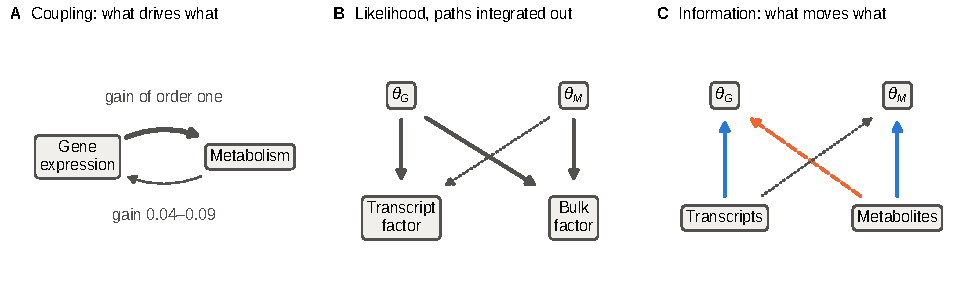
\includegraphics[width=\linewidth]{fig_graphs.pdf}
\caption{\textbf{Three graphs of one model.} A: the coupling is two-way, with a strong drive
from gene expression to the pools and a weak one back. Line width shows gain. B: once the
paths are integrated out, the gene-expression parameters $\theta_G$ enter both factors,
and the metabolic parameters $\theta_M$ reach the transcript factor only weakly (dotted). C:
what the data move. Solid: each stream informs its own module, on both routes. Dashed: metabolites
to gene expression, shown by the linearised bound and the mixed route, with no exact result.
Dotted: transcripts to metabolism, a null read-off on M0.}
\label{fig:graphs}
\end{figure*}

The strength of each coupling direction predicts where information flows
(\cref{tab:gain}). From gene expression to the pools the gain is of order one. The
pools turn over in seconds to minutes, and the drains from gene expression are a
large part of that turnover. From the pools back to the rate constants the gain is
small: an elasticity of \pn{gain.txlo}--\pn{gain.txhi} for transcription and
\pn{gain.tl} for translation. The gain is small because the published rate laws are
saturated. The elasticity here is $\partial \ln k / \partial \ln c$, of a rate constant $k$ in a pool $c$. The published law's dissociation constant $K_d$ for RNA polymerase and its nucleotides is \pn{gain.kd}\,mM, while ATP is near \pn{gain.atp}\,mM.

\begin{table}[t]
\caption{\textbf{Gain and information in each direction across the boundary.} Information is the ratio of posterior to prior standard deviation at 200 cells. The ptsG value is a linearised bound at 10\% assay noise, and its bracket is the ratio that noise alone gives. The ENO value limits what transcripts can inform, since they are a function of the path: a Gaussian approximation from the path's Fisher information, linearised at one truth, from 40 cells scaled to 200, with no assay noise.}
\label{tab:gain}
\centering
\small
\begin{tabular}{@{}P{0.3\columnwidth}P{0.27\columnwidth}P{0.33\columnwidth}@{}}
\toprule
Direction & Gain & Information \\
\midrule
Gene expression $\to$ pools & order one & ptsG from metabolites only: \pn{info.ptsg} (bracket \pn{info.ptsgbracket}) \\
Pools $\to$ rate constants & \pn{gain.txlo}--\pn{gain.txhi} (transcription), \pn{gain.tl} (translation) & ENO from transcripts only: \pn{info.enotx} \\
\bottomrule
\end{tabular}
\end{table}

\paragraph{Metabolites to gene expression.} The linearised bound says that metabolite data can inform the ptsG promoter, a
gene-expression parameter that they never measure. On M0 the mixed route shows this
shrinkage, to \pn{mix.ptsgbulk} of the prior standard deviation. That is less shrinkage than the bound of \pn{info.mzeroptsg} projects, and that calculation's own split-half noise ratio is \pn{info.mzerobracket}. The exact fit under metabolites only did not mix for
this parameter, so on the exact sampler this direction is unmeasured, and we do not claim
it there.

\paragraph{Transcripts to metabolism.} Transcript data carry almost no information about the enolase constant, a
metabolic parameter. We report that result as a null, not as a failure. On M0 at \pn{mzero.cells} cells, the exact sampler's divergence under
transcripts only is \pn{tsplit.eno}\,nat for enolase and \pn{tsplit.fba}\,nat for
aldolase, each below its noise floor. That read-off is M0's. We did not run the
planned test at 1,000 cells, so we do not extend it to the full reduced model.

\paragraph{One data stream at a time, by both routes.} On the reference dataset under transcripts only,
none of the five marginals we compared differs detectably between the routes: the
Wasserstein distance is \pn{mix.txlo}--\pn{mix.txhi} exact standard deviations, each
below its noise floor. The decay rate's posterior variance shrinks by \pn{mix.krnadegtx}\% under transcripts only:
the autocorrelation in a time-resolved single-cell record separates it from the promoter
strength, where RNA-seq data inform only the product of synthesis rate and half-life \cite{karr2015summary}.
Under metabolites only, enolase, the decay rate and $\sigb$
differ detectably, by small margins, and aldolase does not. The exact fit has an
effective sample size of only \pn{mix.krnadegess} for the decay rate. Each floor is one sample of the
noise, so these margins are not precise, and we have not tested whether they share a
cause with the gap of \cref{sec:posteriors}.

